\chapter{Implementation} \label{chap:implementation}

This chapter presents the final implementation of the project. The full process for both the end-to-end event classification models, as well as the two-phase video reconstruction networks are given, alongside any data pre-processing that was required.

\section{Data Preprocessing}

As described in  \cref{ssec:data_preprocessing_design}, data had to be centered to give a z-score. In practice the standard deviation was not used to normalise the values, and instead the following operation was undertaken: $ \textbf{x} = \frac{\textbf{x} - mean_x}{max_x} $. However, during the implementation of the networks it was evident that the default Keras functions would not be ideal. The reason for this is that the dataset, as real-world data often is, were far too large to store on the RAM of a computer. This is the case even with the high-RAM run-times of Google Coloboratory. This meant that data had to be read into the network on a per-batch basis, making the whole process less RAM intensive. Keras has a \lstinline{Sequence} class that can be extended to create a custom data-generator class. \color{red} TODO: Maybe put code example here. \color{black}

\section{End-to-end Event Classification Pipeline}

\subsubsection{Frame Integration}

In order to begin analysing neuromorphic data, it was pre-processed it into a form that a NN can take as input. For most the testing an implementation of the more formal method of processing events streams to get integrated frames given in \cref{ssec:frame_integration} was implemented. This technique was also applied to another readily available data-sets, the DVS128 Gesture dataset.

The integrated frames of a hand gesture in \cref{fig:dvs128_integrated_frames} shows the motion of an arm moving in a clockwise direction \color{red} TODO: Show classic frame integration for NMNIST dataset \color{black}. For each instance of a gesture the event stream was split into 20 frames. This made the processing of the data easy for some of the networks described later in the chapter, since the frames could be packed into 3D tensors of equal size. This means that the frames are not synchronous like they would be from an frame-based camera, and the amount of time represented by each frame is varying. As well as this, since the event streams are of varying length in the time dimension, some videos are reconstructed to a more granular scale than others. It is apparent that in this particular sample a relatively large amount of time is being compressed into every frame, resulting in a large amount of motion being visible. With more frames being created for each sample this problem would be alleviated and more easily distinguishable features may be seen. However if too many frames are taken, not only are processing times greatly increased, events may be sparse and not show any visible pattern in any one frame. A benefit of having this blurring event in the intensity frames is that the direction and degree of motion can be seen in the frames, and so the networks can also pick up these patterns in their classification process.

\begin{figure}[htb]%
    \centering
    \subfloat[\centering]{{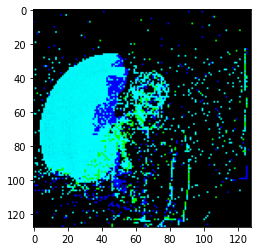
\includegraphics[width=0.25\textwidth]{implementation/images/Dvs128_integrated_frame_1.png}}}%
    \qquad
    \subfloat[\centering]{{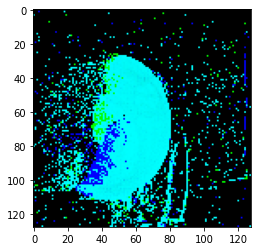
\includegraphics[width=0.25\textwidth]{implementation/images/Dvs128_integrated_frame_2.png}}}%
    \qquad
    \subfloat[\centering]{{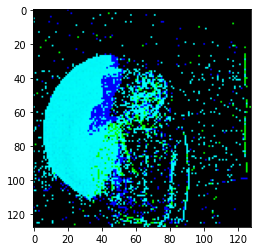
\includegraphics[width=0.25\textwidth]{implementation/images/Dvs128_integrated_frame_3.png}}}%
    \caption{Three contiguous intensity frames \textbf{(a)}, \textbf{(b)} and \textbf{(c)}, created from the DVS128 Gesture dataset with a person moving their right hand clockwise.}%
    \label{fig:dvs128_integrated_frames}%
\end{figure}

\color{red} TODO: Add more photos of integrated frames with more and less frames \color{black}

\color{red} TODO: Add pseudocode for frame integration \color{black}

\subsubsection{Custom Frame-Integration}

As well as this a novel integration technique was implemented, as described in the \cref{sec:end_to_end_classification_design}. The method involved segmenting the events into groups based on their timestamp. \Cref{fig:nmnist_spikes_to_intensity_map} shows a visualisation of intensity maps created from the NMNIST\cite{NMNIST} dataset \color{red} TODO: Show custom frame integration of DVS128 Dataset \color{black}. The set of all events was split into eight segments, where each segment included events within a range of $ 1 \times 10^6 $ ms (i.e., $ 0 \rightarrow 1 $, $ 1 \rightarrow 2 $, ..., $ 7 \rightarrow 8 $). This way the data representation shifted to somewhat get back to a set of frames that mimicked the video output usually seen from everyday cameras. \textbf{(a)} shows the segmented events visualised in three dimensions (x\_location, y\_location and timestamp). In \textbf{(b)} these events were projected onto the two dimensional plane (of x\_location and y\_location), then the plots for on events and off events are shown separately. Finally in \textbf{(c)} an intensity map was created from the projected events. Each pixel in the intensity map grid was initialised to 0, and for every on event 1 was added to the cell, and for every off event 1 was subtracted from the cell. This way temporal information was retained to a greater degree than if each pixel simply had binary information of whether a event occurred or not in a two channel image (as was done by the spikingjelly package\cite{SpikingJelly}). It was clear that the resulting output greatly resembled the MNIST\cite{MNIST} sample recorded by the ATIS camera (As shown in \cref{fig:nmnist_spikes_visualisation} in \cref{sec:existing_datasets}). Another method that aimed to preserve temporal resolution was proposed by Lo\"ic Cordone \textit{et al.}, who proposed `voxel cubes'\cite{MiniVovelCubes}. For this method there were still binary events in every channel, but there were more than two channels so that the events in each time-slice could be subdivided into each channel. When compared to this method, the temporal information can be stored in the same way with the new proposed method, while keeping data size small since it is just a one-channel image. 

\begin{figure}[htb]%
    \centering
    \subfloat[\centering]{{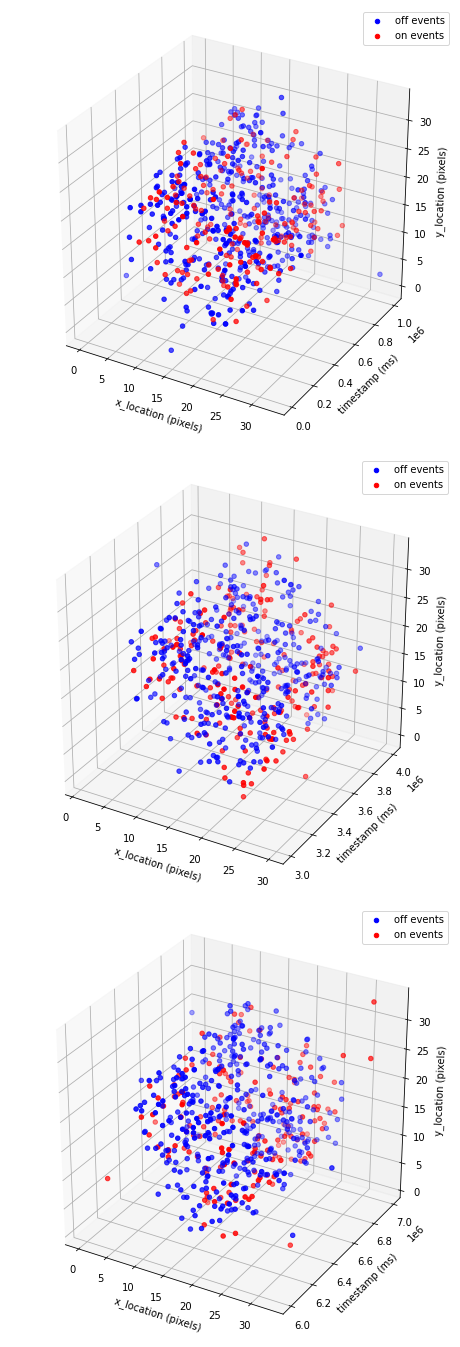
\includegraphics[width=0.25\textwidth, height=0.7\textwidth]{implementation/images/nmnist_spikes_visualisation_segmented.png}}}%
    \qquad
    \subfloat[\centering]{{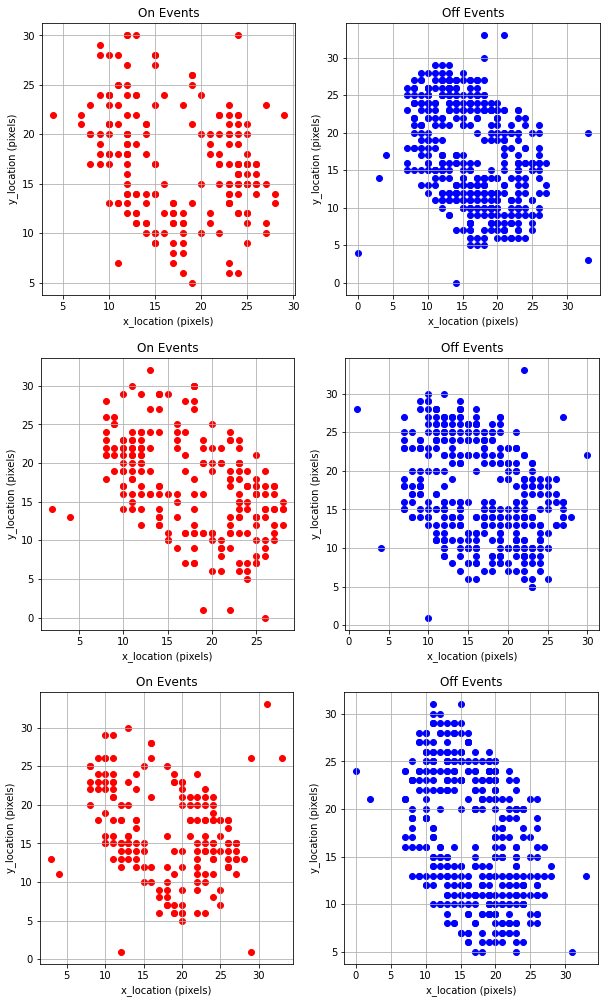
\includegraphics[width=0.4\textwidth, height=0.7\textwidth]{implementation/images/nmnist_events_segmented.png}}}%
    \qquad
    \subfloat[\centering]{{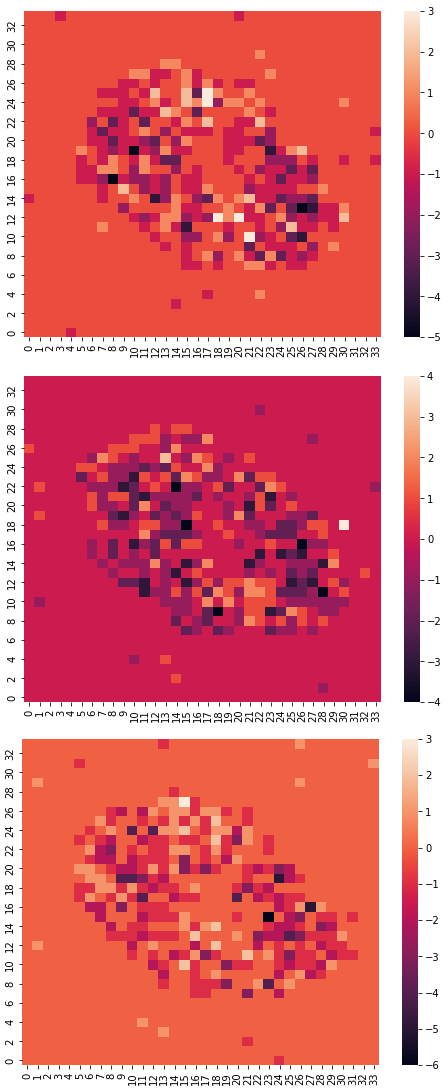
\includegraphics[width=0.25\textwidth, height=0.7\textwidth]{implementation/images/nmnist_events_heatmap_segmented.png}}}%
    \caption{A visualisation of intensity maps created by segmenting events into bins of size $ 1 \times 10^6 $ ms.}%
    \label{fig:nmnist_spikes_to_intensity_map}%
\end{figure}

\color{red} TODO: Add stuff about possible nlp-like networks. \color{black}


\section{Two-phase Intensity Reconstruction Pipeline}

The models described above allow for the system to learn directly on the spiking data. Another approach that was taken was to attempt to utilise video reconstruction networks to the event data so that more classical models and architectures could be used to patterns in the data.

\subsection{Reconstruction Algorithms}

\subsubsection{E2VID}

E2VID, as described in \cref{ssec:video_reconstruction}, is a state-of the art network based on UNET that reconstructs intensity videos from events data. Having gotten the output from the network (which on test data had an average Mean-Squared Error (MSE) of 0.05), it now needed to be processed slightly in order to work with the classification models. The main issue with the reconstruction was that the video were of varying lengths. In order to mitigate this additional frames were added to videos which had fewer frames than that of the longest video in the training set. These additional frames were added by repeating the video until the desired number of frames was reached.

\color{black}

\section{Classification Models}

The models used to classify the either the integrated frames or video reconstructions are given below. Please note that the input shapes given below are for the NMNIST dataset, however for the other datasets different input shapes would be required (e.g. {128, 128, 2} for the DVS128 Gesture dataset).

\subsection{3D Convolutional Neural Network}

The 3D convolutional neural network in \cref{ssec:3D_conv_network} was altered to have the outputs of the hidden layer fed into a dense layer with 10 neurons to classify the correct class (0-9). Activation functions need to be present in the network to prevent all the layers from becoming equivalent to a single one (linear regression model). In order to learn more complex patterns activation functions are a necessary aspect of creating an artificial neuron (See \cref{eq:artificial_neuron_output} in \cref{ssec:snn_and_heterogeneity}). The most commonly used activation function in deep networks (and image recognition in particular) is ReLU, so that was the natural choice for this network as well. Finally, the output layer has a sigmoid activation function. This function compresses the output smoothly between the ranges of 0 and 1. this means each of the outputs from the neurons can be interpreted as a the probability of the input being any one of the 10 classes. This means we can simply take the highest probability as the predicted class from the network.

In order to choose the most appropriate parameters for the system, as well as the other systems implemented during the course of this project, multiple tests were run varying each of the possible hyper-parameters. The tests conducted were to determine;

\begin{itemize}
    \item The number of hidden layers.
    \item The number of neurons per layer.
    \item The size of convolution kernels.
    \item The introduction of some fully connected layers after convolutional layers.
\end{itemize}

The network in each case was trained for multiple epochs. The performance of a typical network can be seen in \cref{fig:accuracy_and_loss_per_epoch}, where the performance on the training set steadily improves as the network progresses through epochs. Accuracy is one of the metrics defined in \cref{sec:evalutaion_metrics}, and the loss for the given network is called categorical cross-entropy loss. The formula used to calculate the loss is given by: $ L = -\frac{1}{N}\sum^N_{i=1}\sum^C_{c=1}y_c^{(i)}log(\hat{y}_c^{(i)}) $, where there are $ N $ samples and $ C $ classes. $ y_c^{(i)} $ is $ 1 $ when the class is correctly predicted and $ 0 $ otherwise and $ \hat{y}_c^{(i)} $ is the predicted probability of class $ c $ for data-point $ i $. This is the same loss function that was used in the other networks in the report as well.

\begin{figure}[htb]
    \centering
    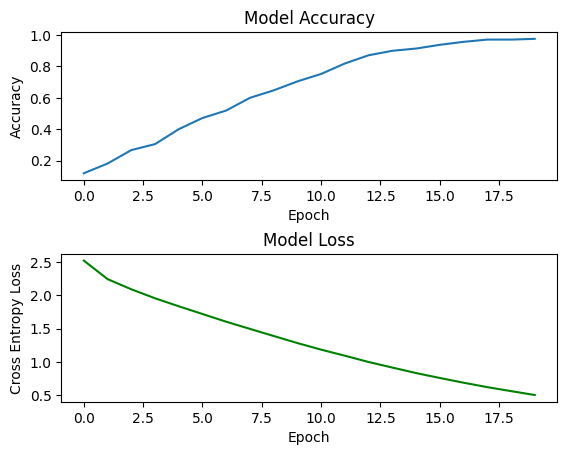
\includegraphics[width=0.4\textwidth]{implementation/images/accuracy_and_loss_per_epoch.png}
    \caption{A figure showing classification accuracy and cross-entropy loss per epoch on training data for a typical network.}
    \label{fig:accuracy_and_loss_per_epoch}
\end{figure}

It was clear, however, that these results may be misleading since they only represent the efficiency of the system when classifying values within the training data-set. However, when looking at the performance on an unseen test data-set, it is obvious that some of the features learnt do not easily translate to general trends in unseen data. This is known as over-fitting, and can be avoided by reducing the capacity of the data-set so that it does not learn information specific to the training set, or by stopping the training process earlier.

Model capacity is directly correlated to the n$ ^o $ of filters, as well as the number of layers, and as the model recognises more patterns in the training data, so it is important to get the optimum value for the system. The size of the kernels has an effect on the scale of the information picked up by the system. With smaller kernels more local patterns are detected, whereas with larger kernels more global effects can be seen. An example of the effects of changing such hyper-parameters can be seen in \cref{fig:hyperparameter_tests} As for the dense layers at the end of the network, it can be seen that better results were achieved as a result of it since global patterns can be further identified after the data has been processed by the convolution layers that have picked out the most important features.

\begin{figure}[htb]%
    \centering
    \subfloat[\centering]{{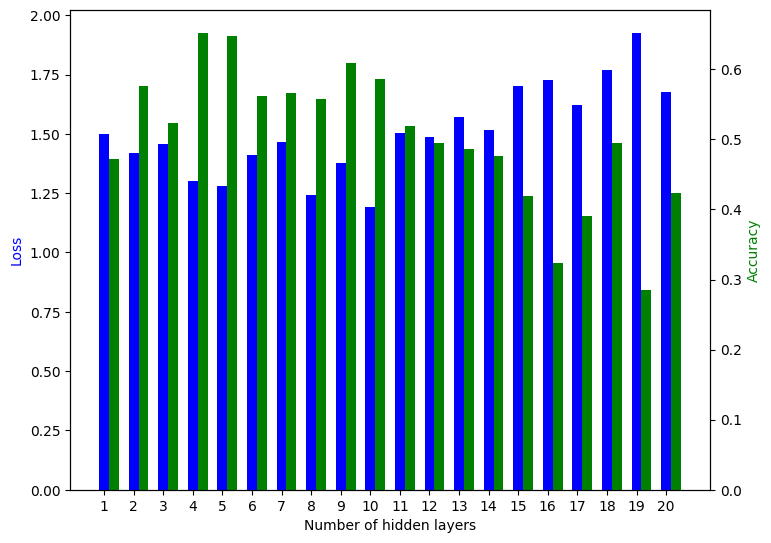
\includegraphics[width=0.4\textwidth]{implementation/images/layer_tests.png}}}%
    \subfloat[\centering]{{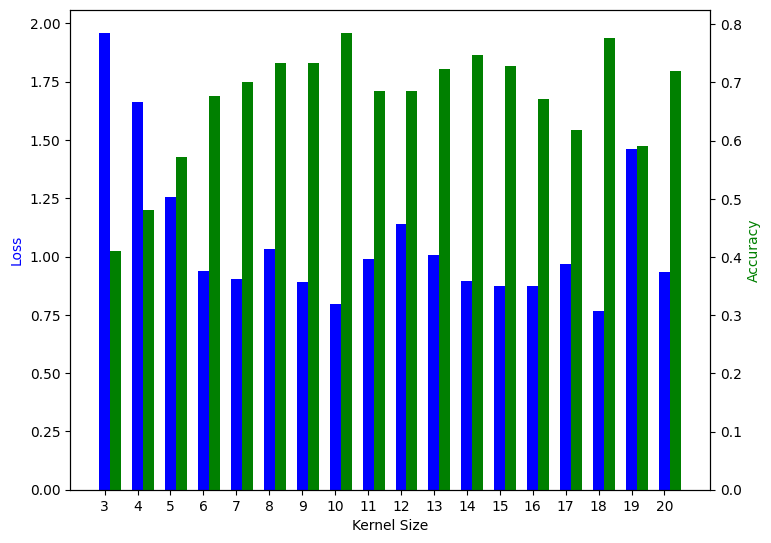
\includegraphics[width=0.4\textwidth]{implementation/images/kernel_tests.png}}}%
    \caption{Graphs showing the effect on training loss with varying hyper-parameters.}%
    \label{fig:hyperparameter_tests}%
\end{figure}

Further testing was done with increasing kernel sizes, and with pooling layers added to the network. 

An overview of the layers present in the network, together with the shape of their outputs and number of trainable parameters can be seen in \cref{lst:3d_conv_layers}. It features the repeating pattern of 3D convolution layers and max-pooling. The number of filters in each layer keeps increasing (from 32 to 64 and 128). The function of 2D filters is to capture patterns in the data, and as you move forward through the network these patterns get more complex. For example, if dots and lines are captured in the first layer, shapes such as triangles and squares may be captured in the second one. Since the patterns are more complex, the number of possible combinations also increases. This is the reason more filters are required for later layers. The max-pooling layers scale down the image, this also means that more large scale patterns can be identified from smaller sections of the frame.

\subsection{Convolutional LTSM}

An overview of the layers present in the network, together with the shape of their outputs and number of trainable parameters can be seen in \cref{lst:conv_lstm_layers}. The thought behind the structure of this network is similar to the one when designing the 3D convolutional network. The number of filters increases as you go further through the network. The difference this time is that 2D convolution is carried out on each contiguous frame of the video input before being passed through LTSM networks. The way this is implemented is with the convLTSM network described in \cref{ssec:conv_lstm}.

\subsection{Custom Convolutional LSTM}

An implementation of a custom convolutional LSTM can be seen in \cref{lst:custom_conv_lstm_layers} and the implementation of the custom 2D convolutional network applied to each frame of the video can be seen in \cref{lst:custom_conv_2d_layers}. This network is the natural progression from the previous convLSTM network since it applies a more complex 2D convolution to each frame. This extra capacity is evident in the number of trainable parameters in the new network when compared to the one in \cref{lst:conv_lstm_layers}.

\subsection{Spiking Neural Network}

For the basis of the spiking neural network, the same 2D convolutional neural network used in the custom convolutional LSTM network (See \cref{lst:custom_conv_2d_layers}). First an ANN was constructed and trained with traditional back-propagation. Since there were a series of frames being input to the network, the actual labels had to be repeated for each frame during the training process. Once this training was complete, the network was converted to a spiking neural network. For this the activation of the neurons in the network were changed from tensorflow's \lstinline{nn.relu} to nengo's \lstinline{SpikingRectifiedLinear}. The specifics for the underlying conversion can be seen in the work done by Bodo Rueckauer \textit{et al}\cite{Ann2Snn}. The neural activity of this network can be seen in \cref{fig:pre_snn_conversion}. The input to this network was a integrated frame video with each frame repeated 8 times (as described in \cref{ssec:snn_design}). The plots are shown over time, and since our network doesn't have any temporal elements (i.e. spiking neurons), the neural activity is for the whole duration it is run. Since the neuron activations are continuous theyH each have a constant rate of neural activity. For this exploratory work the network was trained for 15 epochs, giving an approximate accuracy of 95.62\%.

\begin{figure}[htb]%
    \centering
    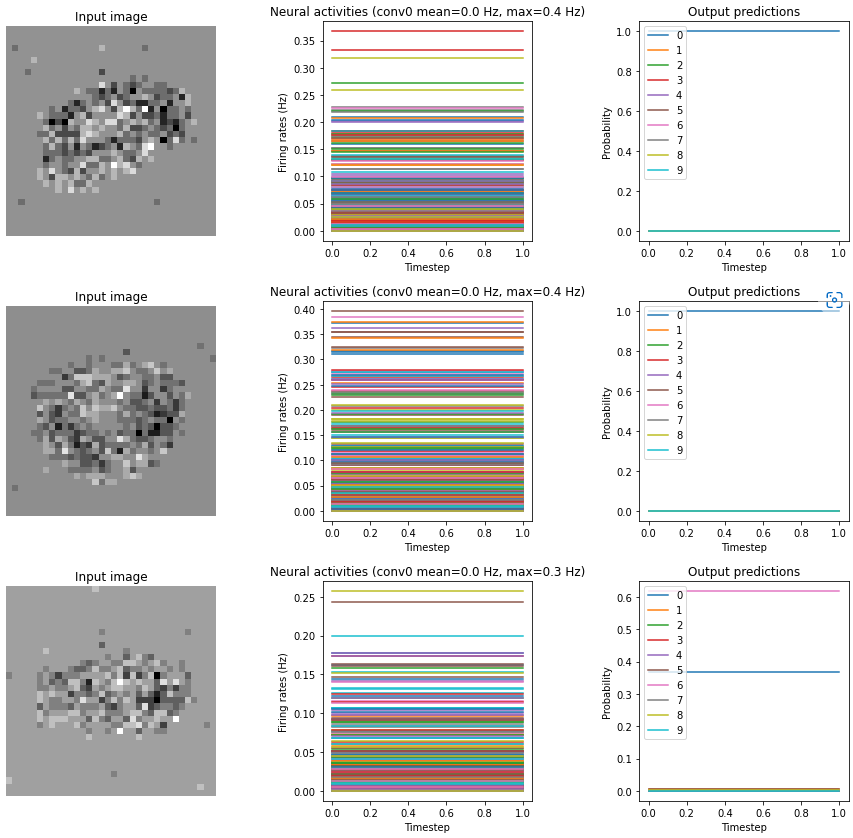
\includegraphics[width=0.6\textwidth]{implementation/images/pre_snn_conversion.png}
    \caption{Graphs showing neural activity of ANN before conversion to SNN.}%
    \label{fig:pre_snn_conversion}%
\end{figure}

Then the network was converted to a spiking neural network by changing the Rectified Linear (ReLU) layers to Spiking ReLU layers. As previously explained, each 3 dimensional vector needed to be sent to the network multiple times to allow for spikes to accumulate in the neural network. It was found that to achieve a good number of spikes in the network the frames had to be repeated 30 times. A graph showing the activity of neurons in the first convolutional layer of the network with high and low number of repetitions can be seen in \cref{fig:frame_repititions}. Graphs showing the performance of the converted network can be seen in \cref{fig:post_snn_conversion}. Note that for this system since data it being passed into it consecutively, the only the final output from the system is sampled for predictions. The accuracy of the converted network fell to approximately 10\%.

\begin{figure}[htb]%
    \centering
    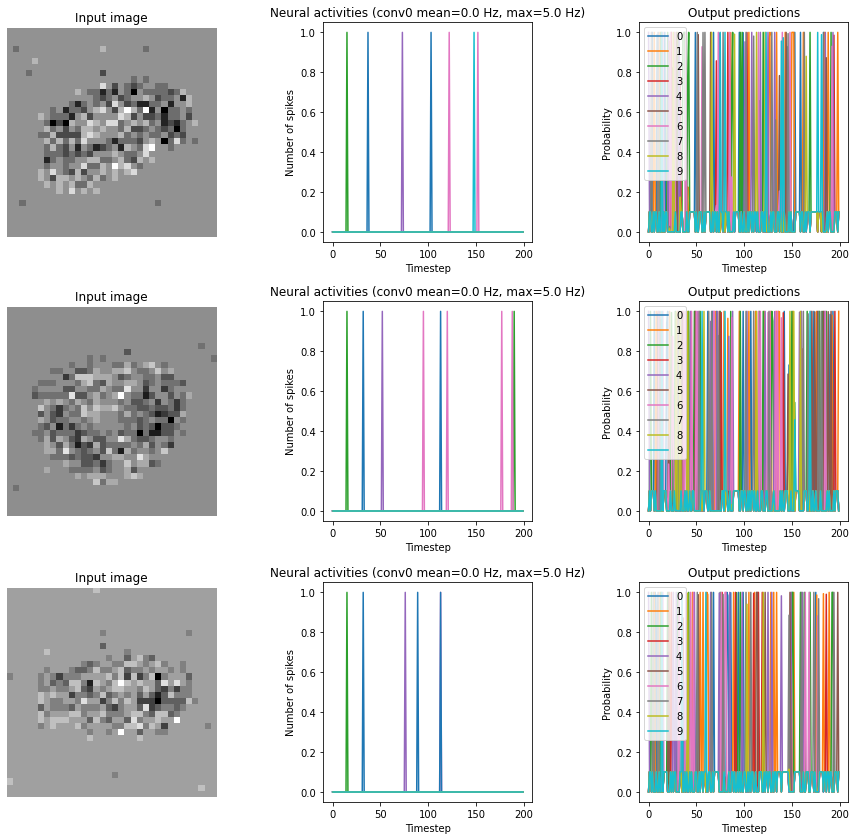
\includegraphics[width=0.6\textwidth]{implementation/images/post_snn_conversion.png}
    \caption{Graphs showing neural activity of ANN after conversion to SNN.}%
    \label{fig:post_snn_conversion}%
\end{figure}

Once the conversion from ANN to SNN was complete, the performance of the network was incomparable to before the process. The reason for this (as outlined in \cref{ssec:snn_and_heterogeneity}) is the poor approximations that take place in the conversion process. In order to mitigate this, some network alterations were made to improve the approximations.

\begin{figure}[htb]%
    \centering
    \subfloat[\centering]{{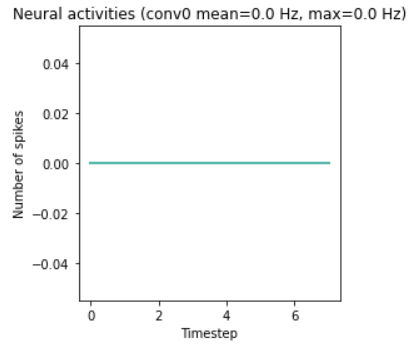
\includegraphics[width=0.4\textwidth]{implementation/images/low_frame_repitition.png}}}%
    \subfloat[\centering]{{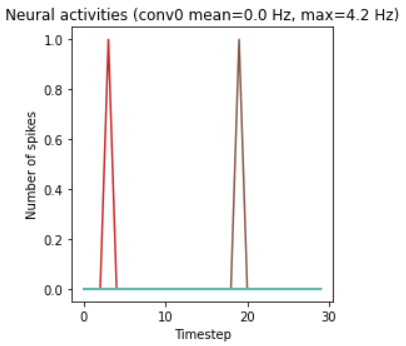
\includegraphics[width=0.4\textwidth]{implementation/images/high_frame_repitition.png}}}%
    \caption{Comparison of number of spikes with less \textbf{(a)} and more \textbf{(b)} repetitions.}%
    \label{fig:frame_repititions}%
\end{figure}

\subsubsection{Synaptic Smoothing}

The plots for the spiking neural network show that since the neuron function is now no-longer continuous, discrete spikes occur to propagate information throughout the network. This means that the output of the network is very noisy. Since there are so many neurons spiking at any one given time, there is no guarantee that when you sample the output at the final time-step that the correct neuron will be firing (even if it has a relatively higher firing rate). For this reason we need to apply a smoothing function to the firing neurons. Essentially the \lstinline{synapse} parameter in nengo applies a moving average filter to the network output so that the predictions are more stable. The effect of applying this filter can be seen in \cref{fig:post_synaptic_smoothing}. It was found that the performance of the system was best with smoothing=0.006.

\begin{figure}[htb]%
    \centering
    \subfloat[\centering]{{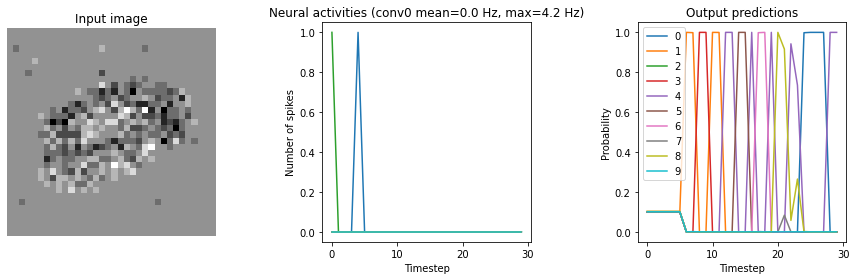
\includegraphics[width=0.4\textwidth]{implementation/images/post_synaptic_smoothing_1.png}}}%
    \qquad
    \subfloat[\centering]{{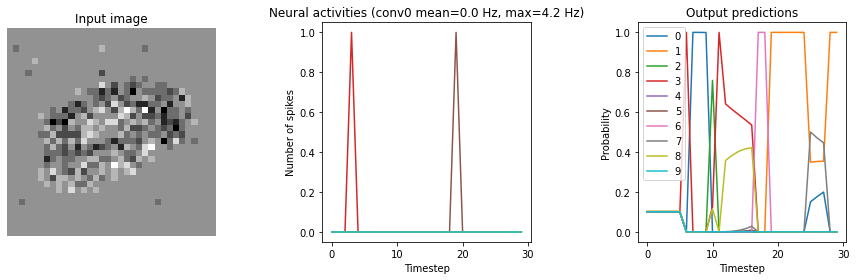
\includegraphics[width=0.4\textwidth]{implementation/images/post_synaptic_smoothing_2.png}}}%
    \qquad
    \subfloat[\centering]{{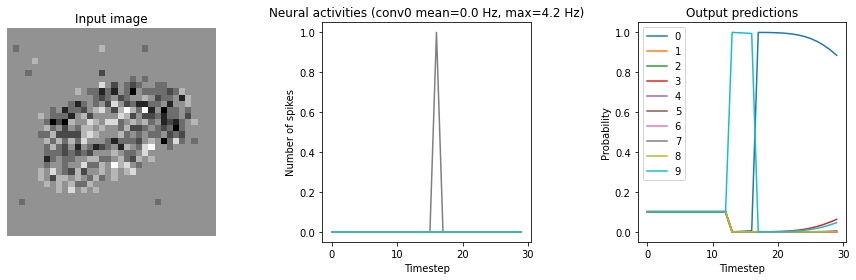
\includegraphics[width=0.4\textwidth]{implementation/images/post_synaptic_smoothing_3.png}}}%
    \caption{Performance of spiking neural network with progressively more synaptic smoothing; \textbf{(a)} smoothing=0.002 \textbf{(b)} smoothing=0.005, and \textbf{(c)} smoothing=0.010.}%
    \label{fig:post_synaptic_smoothing}%
\end{figure}

\subsubsection{Post-training Firing Rate Scaling}

Neuron updates only occur when it outputs, or 'fires' a spike. This means that the system is much more likely to update when firing rates increase. Since the only output function that has been replaces is ReLU, which is a linear function, it is feasible to multiply the inputs of the neurons by a scale factor, then divide the output by the same number to scale. Larger inputs mean the neuron is more likely to spike, yet the linearity of the function is maintained by scaling down the output. The effect of applying this filter can be seen in \cref{fig:post_firing_rate_scaling}. It is important to note, however, that if the firing rate were to theoretically be scales infinitely, the neuron functions for be continuous, exactly replicating artificial neural networks. This may be good in terms of efficiency, but negates the point of using spiking neural networks in the first place. It was found that the best compromise for this system was to scale the firing rate by 150, which preserved the benefits of the spiking neural network and also improved accuracy back to the levels before the conversion.

It is also possible to change the effective firing rates of each neuron in the network, we could also add a custom loss function that incentivises a certain firing rate during the training processes as well. The benefit of this is that it can be applied to non-linear functions other than ReLU, but since there is no such function present in this project it need not be implemented.

\begin{figure}[htb]%
    \centering
    \subfloat[\centering]{{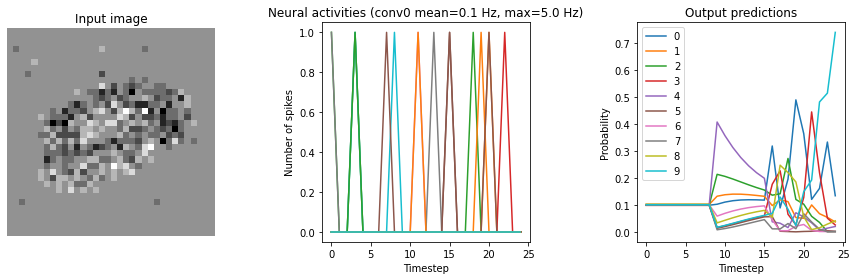
\includegraphics[width=0.4\textwidth]{implementation/images/post_firing_rate_scaling_1.png}}}%
    \qquad
    \subfloat[\centering]{{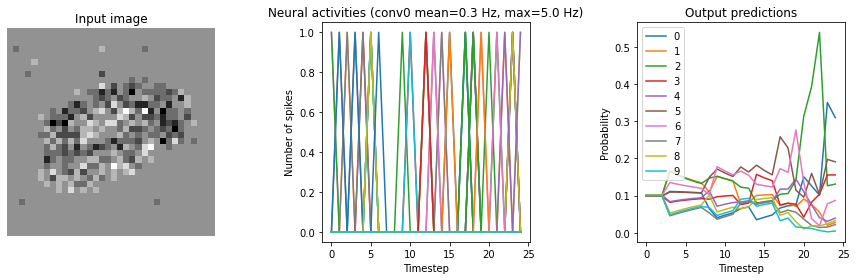
\includegraphics[width=0.4\textwidth]{implementation/images/post_firing_rate_scaling_2.png}}}%
    \qquad
    \subfloat[\centering]{{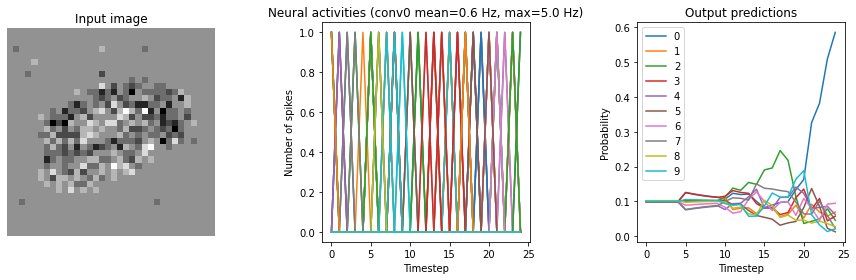
\includegraphics[width=0.4\textwidth]{implementation/images/post_firing_rate_scaling_3.png}}}%
    \caption{Performance of spiking neural network with progressively more firing rate scaling; \textbf{(a)} scaling=20 \textbf{(b)} scaling=50, and \textbf{(c)} scaling=100.}%
    \label{fig:post_firing_rate_scaling}%
\end{figure}